\section{Electrical}

% Goal of the systems

The goal of the electrical systems is to control the experiments and deploy the parachute while collecting as much data as possible about the flight.
We want to be able to test or experiments and make sure everything goes smoothly and be able to do analysis on the results after the launch campaign.
To achieve this the electrical team is working closely with the teams responsible for the subsystems design (air breaks, reaction wheel and parachute).
A member of the electrical goes to the meetings of the subsystems and works with them on the design of the electrical part of their system.

% Managing the experiments
For both the air breaks and the reaction wheel the development of the control software will be handled by the experiment team with help from the software team.
This will allow the experiment teams to test their systems themselves making the testing and tweaking easier.
The role of the software team member will be to make sure that the experiment teams stay within the possibilies offered by the electrical systems.

% Deploying the parachute


% Ground segment

We will now go over each part of the electrical systems one by one, a bloc diagram of their relations is visible on figure \ref{fig:elec_bloc_diagram}.
The arrows represent the flow of data, power flow is not shown.

\subsection{Main computer}

The main computer is made up of the following parts
\begin{itemize}
	\item Control board : We will use a teensy 4.1 as our microcontroller for the main computer.
	\item Sensor inputs : we will have at least a gnss receiver, an IMU and a barometer we are currently finding which exact sensors we will use.
	\item Cameras : 3 cameras each coupled with a \verb+luckfox pico mini+ board will record the flight
	\item Telemetry modules : the data gathered from the sensors and the cameras will be sent to the ground.\\
		We will use LoRa for the sensors data and would like to use VTX for a live video feed.
		We use two different communication systems due to the different constraints and to make sure that we can prioritise the sensors over the camera feed.
	\item Antennas : for antennas we want to use flex PCBs that will be placed on the outside of the rocket tube.
	\item Experiments control : control for the experiments is currently planned to be done from the teensy.\\
		We will research whether having the experiment controls on seperate microcontrollers is better.
	\item Input / Output : The I/O for the main computer will be made up of a small ePaper display (thus visible under bright daylight), a flat joystick and a plug port to connect a laptop.
\end{itemize}

\subsection{Séquenceur}

Nothing special about this, apogee detection will be done using sensors on the main computer, communicated using an optocoupler and the parachute will be deployed.\\
It will have seperate power supply and we will use a buzzer and LEDs for the its output, input is not yet decided.

\begin{figure}[h]
	\centering
	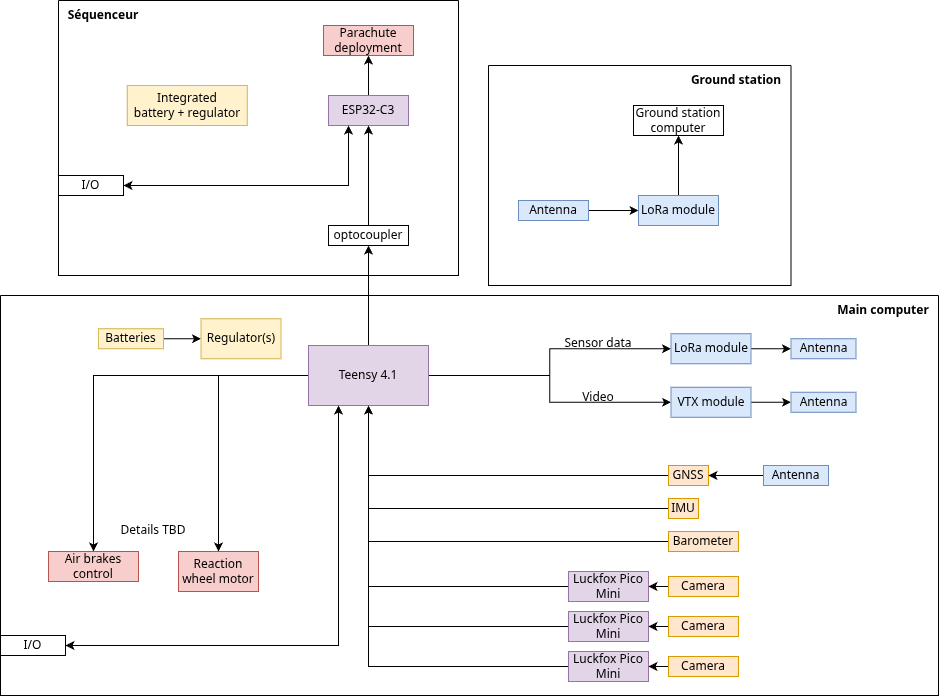
\includegraphics[width=1\linewidth]{elec_diagram.png}
	\caption{Bloc diagram of the electrical systems}
	\label{fig:elec_bloc_diagram}
	\emph{Arrows represent data flow, power not represented.}
\end{figure}

\subsection{Software}

We are currently deciding whether we will use an RTOS or not, we will probably end up using one.

We are in the process of creating a dedicated software team to help write all the code necessary.
This would allow us to do the following which wouldn't be possible (or not as good) without new people
\begin{itemize}
	\item Be able to fully simulate sensor inputs : replace the real sensors with simulated data either software only or with an emulated hardware module.
	\item Design data visualisation software to display the received data live.
	\item Write test suites and modules to do rigorous testing of all code and designs.
	\item Any other things we can think off
\end{itemize}

\subsection{Electrical bay}

Due to the small diameter of the rocket we are designing a multi level bay, each level will be a round PCB and the teensy 4.1 will be placed vertically on the side.
An initial design is visible on the figure \ref{fig:elec_bay}, this is not final and the electrical team will coordinate with the guide rail and the other mechanical teams for integration.

\begin{figure}[ht]
	\centering
	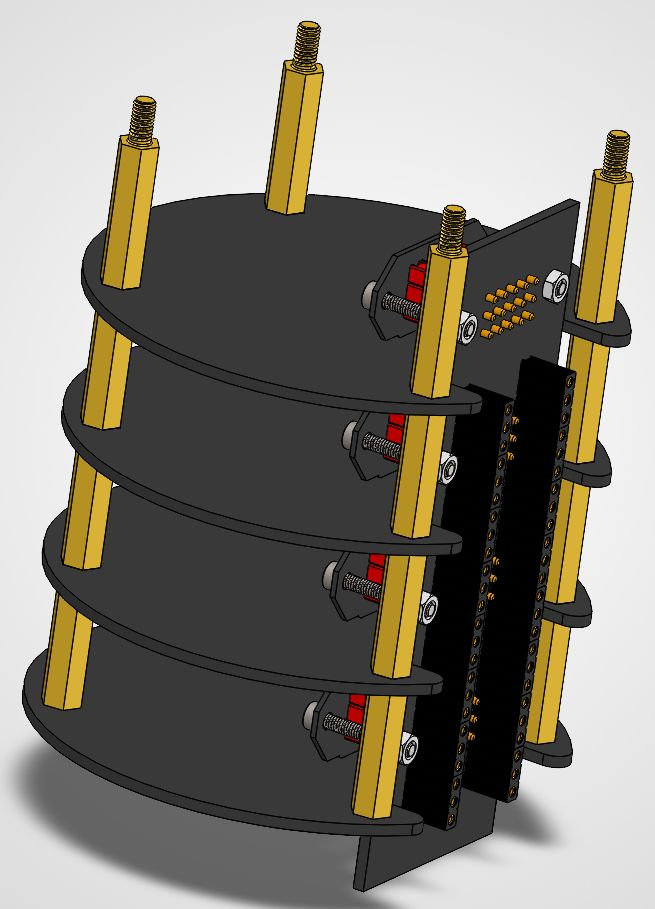
\includegraphics[width=0.8\linewidth]{elec_bay.jpg}
	\caption{First electrical bay draft}
	\label{fig:elec_bay}
\end{figure}


